
\documentclass{sigchi}

%% QUESTIONS FOR CHRIS AND ROB.

%% 1. Is Zooniverse the first citizen science project 
%%    to report scientific findings in research journals?
%% 2. XXX,XXX volunteers, NNN,NNN,NNN classifications
%% 3. ``Guide to social science papers'' - throw me a bone?
%% 
%% TODO for Southampton Team
%% 
%% 1. (for Neal): in intro, zoologists, archaeologists  etc what other
%%     kinds of -ologists?  - Done - See relevant comment under paragraph
%%     3 of introduction.
%% 2. (for Ramine) - Introduction - ``grounded dimension analysis'' - i belive
%% this is a term we made up. Can you re-write this 
%% 3. (for Ramine) - Method - Can you help us get cracking on this
%% 4. (

% Use this command to override the default ACM copyright statement (e.g. for preprints). 
% Consult the conference website for the camera-ready copyright statement.
\toappear{}

% Arabic page numbers for submission. 
% Remove this line to eliminate page numbers for the camera ready copy
%\pagenumbering{arabic}


% Load basic packages
\usepackage{balance}  % to better equalize the last page
\usepackage{graphics} % for EPS, load graphicx instead
\usepackage{times}    % comment if you want LaTeX's default font
\usepackage{url}      % llt: nicely formatted URLs
\usepackage{algorithm,algorithmic}
\usepackage{enumitem}


% llt: Define a global style for URLs, rather that the default one
\makeatletter
\def\url@leostyle{%
  \@ifundefined{selectfont}{\def\UrlFont{\sf}}{\def\UrlFont{\small\bf\ttfamily}}}
\makeatother
\urlstyle{leo}


% To make various LaTeX processors do the right thing with page size.
\def\pprw{8.5in}
\def\pprh{11in}
\special{papersize=\pprw,\pprh}
\setlength{\paperwidth}{\pprw}
\setlength{\paperheight}{\pprh}
\setlength{\pdfpagewidth}{\pprw}
\setlength{\pdfpageheight}{\pprh}

% Make sure hyperref comes last of your loaded packages, 
% to give it a fighting chance of not being over-written, 
% since its job is to redefine many LaTeX commands.
\usepackage[pdftex]{hyperref}
\hypersetup{
pdftitle={SIGCHI Conference Proceedings Format},
pdfauthor={LaTeX},
pdfkeywords={SIGCHI, proceedings, archival format},
bookmarksnumbered,
pdfstartview={FitH},
colorlinks,
citecolor=black,
filecolor=black,
linkcolor=black,
urlcolor=black,
breaklinks=true,
}


% create a shortcut to typeset table headings
\newcommand\tabhead[1]{\small\textbf{#1}}

% End of preamble. Here it comes the document.
\begin{document}

\title{One Does Not `Simply' Launch a Citizen Science Project: Reflections on Zooniverse, a Multi-Domain Science Platform}
% \title{A Brief History of Zooniverse: Designing for Multi-Domain Citizen Science}

\numberofauthors{1} \author{ (Authors removed for reviewing) }
% 
% Rob and Chris: please send me the complete list of authors on your team
% Zooniverse Team: Chris Lintott, Rob Simpson, Arfon (?) 
%   < insert main zooniverse team here > 
% 
% Southampton team: Max Van Kleek, Neal Reeves, Ramine Tinati, 
%   Elena Simperl, Anna Weston, Nigel Shadbolt, Wendy Hall (?)
% 


\maketitle

\begin{abstract}

(( TODO ))

\end{abstract}

\keywords{Citizen science, crowdsourcing, interface design}

%% TODO 
\category{H.5.m.}{Information Interfaces and Presentation (e.g. HCI)}{Miscellaneous}

%% TODO 
%% \terms{}

\section{Introduction}

Web-based ``citizen-science'' projects have enabled hundreds of thousands of untrained human volunteers to contribute to open scientific problems across a variety of domains \cite{citizen-science}.  The handful of successful systems have demonstrated that citizen science applications can be valuable both to participants, as educational tools and cognitively-stimulating puzzles\cite{citizen-science-in-curricula}, as well as to scientific researchers who have large unmanageable data sets and problem spaces \cite{fortson-2011, lintott-08, lintott-11, simpson-12, davis-11}.

% zooniverse et al publications >
% https://www.zooniverse.org/publications 
% http://mnras.oxfordjournals.org/content/424/4/2442.full

% davis-12 : The distribution of interplanetary dust between 0.96
% and 1.04 au as inferred from impacts on the STEREO spacecraft
% observed by the heliospheric imagers, Davis+ 2012.  

% sayighs : Repeated call types in short-finned pilot whales,
% Globicephala macrorhynchus, Sayigh+ 2012.

%However, designing successful citizen science systems that are mutually beneficial in this way and that can successfully sustain participation and useful results over time can be exceedingly difficult.  The reasons are several: first, due to the emerging nature of the field, key design principles and \emph{best practices} are not yet known or established.  Despite considerable overlap with other kinds of human computation-driven systems (e.g., mechanical turk \cite{}), key differences in the ways that participants engage with citizen science online means that these systems have predominantly required 'starting from scratch', to explicitly consider a greater number of design factors, features and dimensions. For example, although human computation systems often apply extrinsic reward schemes to drive participation, such rewards are usually inappropriate for citizen scientists who are predominantly intrinsically motivated to contribute\cite{extrinsic-vs-intrinsic}. However, since the specific motivations that motivate people typically personal and idiosyncratic \cite{raddick2010galaxy}, understanding  ways to address and engage them can be challenging to design for.  Participants typically interact with with citizen science systems in many different ways beyond merely performing tasks, such as by taking part in discussions, interacting with the science teams, sharing subjects they found interesting, and so forth. meaning that measuring 'success' itself can be diffficult.  Finally, the simple fact that, over time, the more time has elapsed simply forget about any particular system, means that retaining experienced particpants over time.

However, it can be extremely difficult to design successful citizen science systems that can achieve this mutually beneficial characteristic and that sustain participation over time.  The reasons are several: first, despite similarities with other kinds of human computation-driven systems, such as typical crowd-sourcing platforms like Amazon Mechanical Turk\footnote{Amazon Mechanical Turk \url{www.amazon.com/mechanicalturk}} or CrowdFlower\footnote{CrowdFlower \url{crowdflower.com}}, participants typically interact with with citizen science systems in many ways beyond performing tasks, such as by taking part in discussions, interacting with the science teams, sharing subjects they found interesting, and so forth.  These many ways that participants engage with citizen science systems reflects the many, varied, and often idiosyncratic motivations behind their reasons engaging with them, the landscape of which is still only starting to be understood \cite{raddick2010galaxy}.  % Designing to engage citizens along these many, personal reasons for participating requires an understanding of these motivations, the activities they foster, and ways to support these activities.

Even when such considerations have been made, citizen science systems can fail for many reasons.  Often, these are due to factors essentially out of the control of the system designer; for example, for some projects, task domain/subject matter is simply  perceived as more interesting to the general population than others.  In some cases, the subjects or tasks may be perceived as unpleasant and off-putting - such as, for example, the identification of tumour cells or mapping of parasites in the tissues of living patients.  Other factors could include the precise ways a project is announced or launched, or the ways and channels used to subsequently promote it.  The combination of these factors means that designers must both cope with a high-dimensional, complex design space that is difficult to explore, and outcomes that are quite unpredictable and uncertain (e.g., \cite{bentham, museums, beamartian}).

% elena notes: 
% some domains are more boring than others, worms versus galaxies
% some domains are dangerous -- 

%, to explicitly consider a greater number of design factors, features and dimensions.  understanding  ways to address and engage them can be challenging to design for.  meaning that measuring 'success' itself can be diffficult.  Finally, the simple fact that, over time, the more time has elapsed simply forget about any particular system, means that retaining experienced particpants over time.

% we want to switch this from interviews to (in crowd). 
% TODO - Ramine - please update this ``retrospective reflective inductive...''
% to something that makes sense - we sat as a group with key team mebers and identified
% themes

In this paper, we contribute a detailed case-study of a citizen-science platform called \emph{Zooniverse} \footnote{Zooniverse - \url{www.zooniverse.org}}, which expanded from a single domain experiment to a  ``factory for citizen science'', an authority for generating successful web applications for researchers across many domains.  After successfully launching their first citizen-science project for astronomy, \emph{Galaxy Zoo}, the team worked closely with zoologists, archaeologists, astronomers, cell biologists, marine biologists, ecologists, biologists, climatologists, geneticists, classicists and historians to produce 27 citizen science projects as of September 2013.  This has given the Zooniverse team a unique perspective on the many variations of needs pertaining to citizen science problems, and extensive experience in designing and deploying such systems in production. These projects followed an evolutionary, iterative design process, applying insights derived each project to the next.  Some projects were re-designed and re-launched several times using ideas and experienced gained from the others.   This iterative process has allowed the Zooniverse team to explore design decisions at multiple levels, from aspects of the interface and interaction flow, to social elements (such as discussion forums), to strategies towards attracting potential users and sustaining prolonged engagement. 

% 

%  The diversity of projects required different scientific domains, as it involved working closely with zoologists, archaeologists, astronomers, cell biologists, marine biologists, ecologists, biologists, climatologists, geneticists, classicists and historians, among others.

 % Zooniverse also represents the first system in which volunteer contributions directly resulted in the publication of scientific findings in academic journals, contributing findings to at least $P$ published scientific papers.  

% Zooniverse projects are of benefit to zoologists, archaeologists, astronomers, cell biologists, marine biologists, ecologists, biologists, climatologists, geneticists, classicists and historians(and potentially others as well, from retired projects)

In this paper, we summarise the results of a retrospective reflective thematic analysis conducted with core members of the Zooniverse team, to identify the key design decisions that were made, and to document the informal knowledge gained from their process.  This was done primarily to allow perspectives on this complicated design space to be shared with both UX practitioners interested in designing for citizen-science, as well as to contextualise these design dimensions against the growing crowd-sourcing and online community studies being in the HCI research community.  

We begin with a short history of the project in order to introduce readers with the context for the following discussion, followed by a dimensional design analysis of particular aspects of Zooniverse's deployment.  Finally, we discuss Zooniverse's team's perspective of the greatest difficulties for building more effective citizen science: $X$, $Y$ and $Z$, and ways that HCI research may be able to help.

% maybe a tad redundant:
%% The goal of the this paper is to, first, document the informal knowledge gathered by the Zoonvierse team pertaining to how to design successful citizen science projects, based on their experience of launching 27 projects since the platform's genesis.  These insights are then discussed in the greater context of human computation, to derive design recommendations and discuss factors that may be responsible for the observations made. We begin with a short history of the project in order to provide readers a context for the following discussion, followed by a grounded dimensional design analysis of particular aspects of Zooniverse's deployment.  Finally, we discuss Zooniverse's team's perspective of the greatest difficulties for building more effective citizen science: $X$, $Y$ and $Z$, and ways that HCI research may be able to help.


\section{Background: A Brief History of the Zooniverse}

%% OUTLINE from Rob >> #TODO turn into a timeline (eMax)
%% After Galaxy Zoo it was clear that more projects were to follow.
%% In develping GZ2 Arfon Smith created `Juggernaut' a Ruby on Rails application, with a MySQL back end, designed as a generalised web application for citizen science projects like Galaxy Zoo.
%% %% Neal this is when the ideas of annotations, classifications etc came into being

% Terminology of Zooniverse 
% See blog post by arfon > 
% The Zooniverse team have developed a shared vocabulary for discussion
% of the system, which resulted from knowledge gained throughout $5$
% years of project building as well as patterns resulting from working
% with science teams.

% \emph{Users} are the volunteers using the system. Each user entity
% consists of a username, email address, information about the projects
% they've used and other related pieces of information.

% \emph{Subjects} are the individual assets which users are shown when
% classifying. They may consist of images, audio files or videos.

% \emph{Tasks} are the activities which users carry out when presented
% with a subject.

% \emph{Workflows} are groups of tasks.

% \emph{Classifications} are made up of the user, subject and task
% entities.

% \emph{Groups} are groups of subjects - Subjects from a particular
% time period or 'season' in the Snapshot Serengeti project  may form 
% a group, for example.

% \emph{Projects} are overarching entities with which subjects, groups
% and classifications are associated. In the Ouroboros API used by 
% Zooniverse, project entities store information about groups and the
% status of the project, as well as other administrator functions.

%% Early 2010 saw Solar Stormwatch happen, a project effectively built for someone else (Royal Observatory Greenwich) by the Zooniverse. It used Juggernaut and is still running.
%% <<When does the CSA happen!?>>
%% October 2010 sees the deployment of Old Weather - the first non-astronomy project, first transcription project and first to incorporate any game mechanics.
%% Around the same time we began to take social media more seriously and created a blog network, Twitter/Facebook accounts and even held special events such as the (now annual) Zooniverse Advent Calendar in Dec 2010.
%% The Milky Way Project and Planet Hunters launche din Dec 2010 both using public astronomy datasets (like Galaxy Zoo).
%% In July 2011 Anicent Lives launches - another non-astronomy, transcription project.w
%% In August 2011 we created `Talk' as a way to begin to better harness the power of our discussion fora. The PHP fora we used beforehand were beocming difficult to support and hard to mine for data. We felt that there was a better user experience to be created and a better way for citizen scienceto happen, base don the experienc eon the Peas Corp and the stor yof the Voorwerp.
%% In August 2011 Ice Hunters went live. Built by a separate development team using our system.
%% In Oct 2011 NEEMO was our first purely experimental project - where we weren't even sure of the scientific outcome. We were very clear about this with the users and even housed it in a new `labs' area of the Zooniverse site to be clear that it was an experiment.
%% Whale FM (Nov 29 2011) was our first project to use sound. It was clear early on that it wasn't as popular as the others.
%% In January 2012, BBC Stargazing Live featured Planet Hunters and we received a million classiciations in just two and a bit days. Planet Hunters was actually more popular in the days following the announcement of our discovering a planet during that time, that it had been during the BBC show.
%% In early 2012 we came up with the idea of switching to MongoDB and HTML5 web-apps served from Amazon S3 buckets. The new system: `Ouroboros' would replace Juggernaut and act as a one app serving all our projects. The Juggernaut codebased had become fragmented and each project required its own server and DB. It was getting expensive! IN Sep 2012 we ran `Citizen Science September' and launch four projects in four weeks. These were all base don the new system and it worked out very well.
%% BBC Stargazing returned and in Jan 2013 we launched Planet Four, built specially for the show.
%% AT writing, the latest project was Worm Watch Labs, the 27th project launched in June 2013.

\begin{table*}
\begin{center}
\small
\begin{tabular}{lcllclll}
\hline
Project & Status & URL & Launch & Category & Logged-In & Assets & Interface \\
Name &  &  & Date &  & Users &  &  Type \\
\hline
\hline
Galaxy Zoo & Retired & zoo1.galaxyzoo.org & 11 Jul 2007 & Space & 165,000 & 890,000 & Classification \\
\hline
Galaxy Zoo 2 & Retired & zoo2.galaxyzoo.org & ?? ??? 2009 & Space & XX,XXX & 304.122 & Classification \\
Galaxy Zoo Mergers & Retired & mergers.galaxyzoo.org & 23 Nov 2009 & Space & 20,588 & 58,956 & Classification \\
\hline
Solar Stormwatch & Active & solarstormwatch.com & 22 Feb 2010 & Space & 65,971 & YY,YYY & Classification/Marking \\
Galaxy Zoo Supernova & Retired & supernova.galaxyzoo.org & 26 Mar 2010 & Space & 37,150 & 76,376 & Classification \\
Galaxy Zoo: Hubble & Retired & zoo3.galaxyzoo.org & 17 Apr 2010 & Space & XX,XXX & ~200,000 & Classification \\
Moon Zoo & Active & moonzoo.org & 11 May 2010 & Space & 121,251 & 435,314 & Marking \\
Old Weather & Active & oldweather.org & 12 Oct 2010 & Climate & 32,076 & YY,YYY & Transcription \\
The Milkyway Project & Active & milkywayproject.org & 07 Dec 2010 & Space & 57,675 & 35,695 & Marking \\
Planet Hunters & Active & planethunters.org & 16 Dec 2010 & Space & 167,354 & 3,063,759 & Type \\
\hline
Ancient Lives & Active & ancientlives.org & 25 Jul 2011 & Humanities & 24,983 & 153,885 & Transcription \\
Ice Hunters & Retired & icehunters.org & 09 Aug 2011 & Space & 15,276 & YY,YYY & Classification/Marking \\
NEEMO & Active & neemo.zooniverse.org & 15 Oct 2011 & Space & X,XXX & YY,YYY & Classification \\
Whale FM & Active & whale.fm & 29 Nov 2011 & Nature & 2,150 & 15,531 & Classification \\
\hline
SETI Live & Active & setilive.org & 29 Feb 2012 & Space & 63,609 & YY,YYY & Type \\
Galaxy Zoo 4 & Active & galaxyzoo.org & 11 Sep 2012 & Space & 48,550 & 390,907 & Classification \\
Seafloor Explorer & Active & seafloorexplorer.org & 13 Sep 2012 & Nature & 14,099 & 123,077 & Marking \\
Cyclone Center & Active & cyclonecenter.org & 27 Sep 2012 & Climate & 4,767 & 196,638 & Classification \\
Bat Detective & Active & batdetective.org & 02 Oct 2012 & Nature & 1,580 & 582,203 & Classification \\
Cell Slider & Active & cellslider.net & 23 Oct 2012 & Biology & 13,261 & 275,702 & Classification \\
Andromeda Project & Active & andromedaproject.org & 05 Dec 2012 & Space & 5,072 & 12,425 & Marking \\
Snapshot Serengeti & Active & snapshotserengeti.org & 11 Dec 2012 & Nature & 22,173 & 1,240,727 & Classification \\
\hline
Planet Four & Active & planetfour.org & 08 Jan 2013 & Space & 34,718 & 98,920 & Marking \\
Notes from Nature & Active & notesfromnature.org & 22 Apr 2013 & Nature & 3,490 & 123,402 & Marking/Transcription \\
Space Warps & Active & spacewarps.org & 08 May 2013 & Space & 9,544 & 345,240 & Marking \\
Worm Watch Lab & Active & wormwatchlab.org & 30 Jun 2013 & Biology & 3,251 & 74,016 & Classification \\
\hline
\end{tabular}
\normalsize
\label{project-summary}
\caption{Summary of Zooniverse projects past and present, including each projects status as of September 2013.  The 1.68 million assets in the various Galaxy Zoo projects are not unique, since galaxies in GZ1 were used in subsequent projects.}
\end{center}
\end{table*}

% According to neemo.zooniverse.org, NEEMO had 47,943 user validations, though this may differ from "logged-in users." Particularly because two figures are given - 485 volunteers joined the mission. 

In contrast to crowd-sourcing and citizen science projects that focus on participant-driven data collection (e.g., \cite{okolloh2009ushahidi}, \cite{zook2010volunteered}), the focus of Zooniverse is exclusively citizen \emph{data analysis}, that is, having participants help with the classification, labeling and extraction of information from large, already extant datasets. As documented previously by Fortson et al \cite{fortson2011galaxy}, the first Zooniverse project, \emph{Galaxy Zoo}\footnote{Galaxy Zoo - \url{www.galaxyzoo.com}}, engaged volunteers in the morphological classification of images of galaxies, and launched in July 2007 \cite{galaxyzoo-launch}.  The first scientific papers that resulted from findings from Galaxy Zoo's over 100,000 citizen contributors were published in 2008, on spin statistics of spiral galaxies\cite{land2008galaxy} and the morphological characteristics of galaxies\cite{lintott2008galaxy}.

% Mention Hanny's Verwoop and Green Peas here
The success of Galaxy Zoo 1 generated significant interest, and it became clear that there would be more projects to follow.  The first such project was \emph{Solar Stormwatch}\footnote{Solar Stormwatch - \url{http://www.solarstormwatch.com/}}, effectively built for the Royal Observatory of Greenwich by Zooniverse.  The first non-astronomy project, \emph{Old Weather}\footnote{Old Weather - \url{www.oldweather.org}}, launched in October 2010 and applied volunteers to transcribe historical, hand-written weather measurements from official logs of merchant trading ships from the period of 1780-1830.  As of September 2013, the Zooniverse family of projects has benefited from the participation of $XXX,XXX$ volunteers who have collectively contributed over $NNN,NNN,NNN$ classifications to the system.  

% elena notes:
%   explain 'retired' and 'active', - Also, Andromeda is 'paused,' awaiting data according to the Zooniverse page, (not active)
%   explain 'Type' in 'Interface Type' column
Table 1 lists all of the Zooniverse projects by launch date, along with their current status, their web site locations, sizes of data sets, and task type, as of September 2013.  \emph{Classification} projects ask users to identify the presence, types, and potentially number of things visibile in each subject.  An example of such a task is identifying and counting the number of animals visible in a particular automatically-taken photo, taken by motion-detecting camera in \emph{Snapshot Serengeti}. \emph{Marking} tasks involve the additional step of indicating where in the image the particular object is found, for example, identifying the location of organisms in the undersea images of \emph{Seafloor Explorer}.  Finally, \emph{transcription} tasks involve reading, often deciphering difficult-to-read, text and characters typically from old handwritten texts, such as the ship logs in \emph{Old Weather} or scientists' field notebooks in \emph{Notes from Nature}.    

Figure 1, likewise, illustrates the growth of the project from June 2007 until September 2013. The complete list of scientific papers that have resulted from Zooniverse are compiled on the Zooniverse Blog\footnote{Zooniverse Publications - \url{https://www.zooniverse.org/publications}}.

\subsection{Zooniverse Terminology and Overview}
% elena notes: 
% 'ultimately responsible for the project' - explain this --  zooniverse team were taking over lots of these tasks but now they're providing the tools for the science teams to have more autonomy. 
In the remainder of this paper, we adopt the Zooniverse team's terminology for describing the system and its components, which we briefly summarise here. In the context of Zooniverse, \emph{projects} are proposed to the core Zooniverse team by researchers who become the project's \emph{science team}.  The science team are ultimately responsible for the project once launched.  Each project represents a single, specific line of inquiry and data set, and is launched as a separate web site, with a dedicated discussion forums,  and associated social media channels, including a blog, Twitter account and Facebook page.  Volunteer participants, referred to as \emph{users}, who sign up to any Zooniverse project can contribute to any of the others through links at the top of each Zooniverse project site.  

%% 'asset' in the table -> 'subject' - The table currently appears before the terminology section, so it may be
%% necessary to make clear what subjects refer to prior to this, as this is a somewhat unorthodox usage of 'subject'
Users who are the top contributors may be appointed \emph{moderators}, who are granted special privileges in the discussion forums, and granted access to contacting the \emph{science teams} who ultimately run each project. The term \emph{subject} refers to the individual assets that users are tasked with classifying.  Subjects may consist of images, audio files or videos. \emph{Tasks} are the particular activities which users carry out when presented with a subject, such as identifying the presence and shape of a galaxy in a set of subjects. Subjects are typically organised into \emph{groups}, which represent a particular data set collection, such as those from a particular time period or source such as the Hubble telescope.  Finally, a \emph{Classification} is a single labeling or identification action performed by a single user, upon a subject, within the context of some task, of a project. 

% \subsection{Previous Zooniverse Studies}
% (( TODO : Write up a summary of the social science and systems Zooniverse papers ))

\section{Method}

\begin{figure}[tbp]
\begin{center}
\begin{enumerate}[itemsep=2mm]
\item \emph{What are the most important insights gained through the design process?}
\item \emph{What were your best ideas and worst mistakes?}
\item \emph{Were there any surprises, or unexpected results?}
\item \emph{When you design and launch a new project now, what do you do differently than you would done at the start?}
\end{enumerate}
\vspace{10pt}
\label{tbl:questions}
\caption{\emph{Questions for triangulation} - The interview process started with (and iteratively returned to) these four main questions as probes, to yield the main themes for analysis.}
\end{center}
\vspace{-10pt}
\end{figure}

% triangulation approach?
In order to identify the insights  most valuable to the team from their multi-year iterative design process, we applied a mixed-methods approach drawing upon both quantitative and qualitative sources. The qualitative data collected consisted of four semi-structured interviews were conducted with a selection of members of the Zooniverse Team which included: two designers, the lead project manager, and the team leader. Interviews were chosen as the main source of qualitative data for this study for a number of reasons, they provide a rich and first-hand source of information which can help to draw out insights unlike other sources of qualitative or quantitative data \cite{Yin2003}, to this point, the tacit knowledge that this paper wishes to describe is embedded within the experiences gained within the Zooniverse team members. Interviews provide the unique position where more than one set of experiences and opinions can be discovered, and it is through the triangulation and agreement between data sources that help distill rich insightful \cite{Denzin1978} \cite{Morse1994}. 

The interviews of the four participants were conducted over a serious of eight 2-hour tape recorded sessions. Each participant was asked identical open-ended questions related to their experience in designing, launching, and maintaining the Citizen Science projects which they have been involved in. The interviews were performed in two, 2-hour sessions as part of a reflective process to ensure that the interviewee had had adequate time to describe and reflect on their experiences discussed. Prior to the initial interview session, the participants were asked to prepare any material they wished (in various mediums, i.e. text, video, presentations) which would help them capture the previous 5 years of experience which they have gained during the design, development and deployment cycle of the citizen science projects they were involved with. At the end of the first session, the manually transcribed dialog were given to the participants in order for them to reflect on the experiences which they shared. The second session was then used to discuss these experiences in more detail which were captured in additional notes taken by the researcher. After the second stage of interviews, the transcripts were amended where required, and then anonymised in order to ensure integrity within the coding and elicitation stages of the study. The reflective iterative process used within this study was found to help extract experience and knowledge of the participants which would have remained hidden without the chance for interviewees to comment and discuss their dialog further. It was also found that participants use of material within the were beneficial for helping them recall experiences, especially with regards to the earlier Zooniverse projects.

An iterative manual coding approach was conducted by three researchers to provide the first level of analysis for the interviews. In order to initiate the coding process a topic guide was used which contained a themes related to the questions that interviewees were asked. Each interview underwent a first iteration of coding based upon the codes within the topic guide, and during this process additional themes were identified. this process was performed by the 3 researchers who subsequently cross-compared the additional themes they each found. Based upon an agreement of these new themes and a review of the notes that were taken by the researcher that conducted the initial interview, a new coding schema was developed and the interviews were re-coded in order to extract codes that were missed. This process was repeated for each interview in order to ensure validity and consistency \cite{Strauss1987} \cite{Lafaille1995}. Each researcher also took notes when coding the interviews to describe any comments or discussions that appeared relevant but external to the themes identified. Separate coding of the interviewees were brought together using NVIVO which was then used to extract the relevant information required.

The study also drew upon a mix of quantitative data sources including a dump of the entire Zooniverse discussion and classification database. Included within this were the records for each individual user (anonymised), the classification for (n) difference Zooniverse projects, and the individual comments made of the discussion forums of the respective Zooniverse projects. The purpose of using this mixed methods approach was to compliment and add further insight into the rich qualitative data sources \cite{EdwardsCrossley2009} in order to further unpack and understand the characteristics of producing successful Citizen Science projects.

%% -----------------
% In order to achieve a rich understanding of how successful citizen science is conducted, the study conducted within this research used a mixed methods approach which drew upon both quantitative and qualitative sources of data. The qualitative data collected consisted of four semi-structured interviews were conducted with a selection of members of the Zooniverse Team which included: two designers, the lead project manager, and the team leader. These interviews were conducted over a serious of four 2-hour sessions and each interviewee was asked the same set of open-ended questions related to their experience in designing, launching, and maintaining the Citizen Science projects which they have been involved in. Each interview was recorded, manually transcribed, and then anonymised in order to ensure integrity within the coding and elicitation stages of the study. Interviews were chosen as the main source of qualitative data for this study for a number of reasons, they provide a rich and first-hand source of information which can help to draw out insights unlike other sources of qualitative or quantitative data \cite{Yin2003}, to this point, the tacit knowledge that this paper wishes to describe is embedded within the experiences gained within the Zooniverse team members. Interviews provide the unique position where more than one set of experiences and opinions can be discovered, and it is through the triangulation and agreement between data sources that help distil rich insightful \cite{Denzin1978} \cite{Morse1994}.

%% Such interviews were grounded in following questions:
%% 1. What were the primary design priorities of the team
%% 2. What were the most difficult design decisions of the team
%% 3. What 

% An iterative, manual coding approach was conducted by three researchers to provide the first level of analysis for the interviews. In order to initiate the coding process a topic guide was used which contained a themes related to the questions that interviewees were asked. Each interview underwent a first iteration of coding based upon the codes within the topic guide, and during this process additional themes were identified. this process was performed by the 3 researchers who subsequently cross-compared the additional themes they each found. Based upon an agreement of these new themes, a new coding schema was developed and the interviews were re-coded in order to extract codes that were missed. 

% This process was repeated for each interview in order to ensure validity and consistency \cite{Strauss, 1987} \cite{Lafaille, 1995}. Each researcher also took notes when coding the interviews to describe any comments or discussions that appeared relevant but external to the themes identified. Separate coding of the interviewees were brought together using NVIVO which was then used to extract the relevant information required.

% The study also drew upon a mix of quantitative data sources including a dump of the entire Zooniverse discussion and classification database. Included within this were the records for each individual user (anonymised), the classification for 27 difference Zooniverse projects, and the individual comments made of the discussion forums of the respective Zooniverse projects. The purpose of using this mixed methods approach was to compliment and add further insight into the rich qualitative data sources \cite{Edwards and Crossley, 2009} in order to further unpack and understand the characteristics of producing successful Citizen Science projects.

\section{Dimensions for Design}
% Themes? Observations?

%% sustaining engagement

\subsection{Key components of a citizen science project}

Despite the development of projects in very different domains of academic research, and which involve disparate user interactions, the core requirements for a successful citizen science project remain stable. A `main' interface allows a \emph{user} to complete a \emph{task} when presented with a \emph{subject}. The task is typically constrained by the tools provided (e.g. answer questions from a decision tree, mark craters on an image) and when completed typically results in the presentation of the next subject to be classified. In Zooniverse projects to date, participants perform tasks individually, and are typically not given control over choice of what subjects to work on. This latter choice makes deliberate manipulation of the data difficult and also ensures that project priorities are respected (i.e. it's not just the beautiful/interesting/easy subjects that are worked on). Secondly, some tutorial elements - either as a stand-alone tutorial, as an interactive within the interface or as surrounding context - are required to acquaint users with their tasks. An additional environment for discussion is typically, but not always, provided allowing for more free-form interaction between users and other participants such as scientists, developers and for which work goes beyond the initial task. Extra tools for manipulated subjects or for exploring contextual information may be provided in association with these discussion environments. 

%% One of Arfon's blog posts ties in nicely with the above "despite the development..." as it explains that fundamentally 
%% the team have tried to make it so that each project is the same 'deep down', differing only by goal and interface

A community of participants is implicitly necessary for a citizen science project; crowdsourcing without a crowd is a perhaps unsolvable problem. However, levels of participation and involvement in the community will naturally vary; Zooniverse projects typically receive a substantial number of their classifications from users who will never return. A successful citizen science project will thus be designed to both enable these short-term participants to make useful contributions while still fostering longer-term engagement. This need also illustrates the requirement in most cases to assess the ability or accuracy of participants; many projects thus incorporate `tests', either explicitly or more commonly by including simulated or expert-classified subjects in the workflow presented to users. 

%% The Hcomp2013 "Volunteers' engagement in volunteer thinking project" paper states that for the Milky Way project, 78% of all
%% classifications are completed by regular users (i.e, those who return at least more than once) and for the Galaxy Zoo project
%% this value increases to 80%, which conflicts heavily with the above statements.

\subsection{Task and Tutorial Design}

\subsection{Discussion Forums}

\begin{figure}
\centering
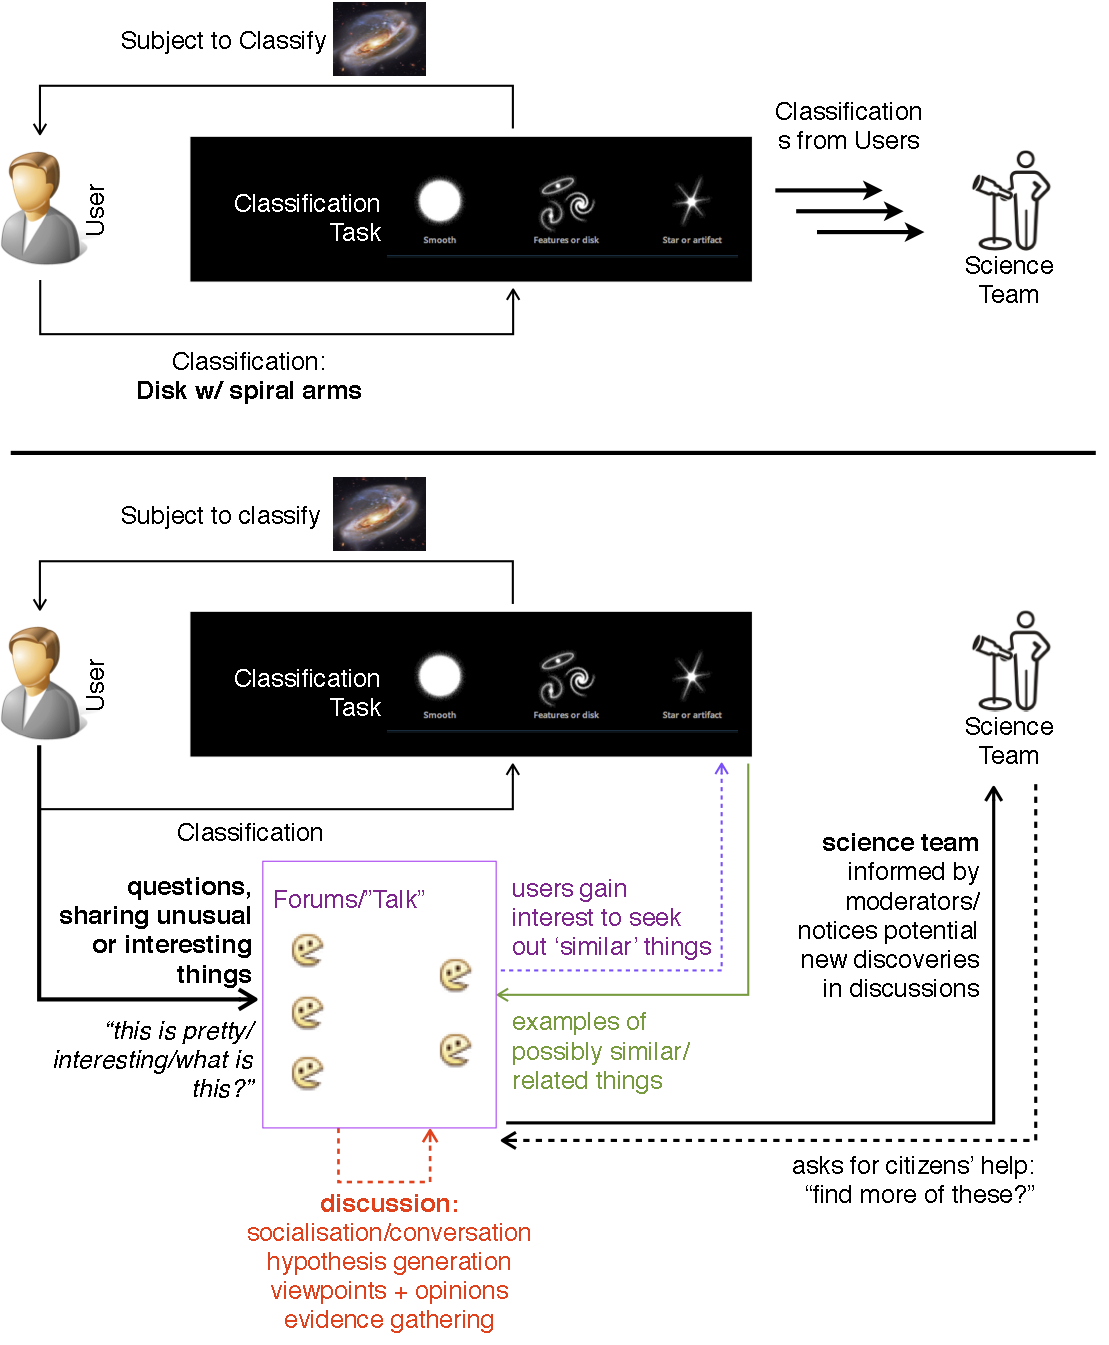
\includegraphics[width=0.48\textwidth]{imgs/twopaths.png}
\caption{\emph{Two paths to science} - In addition to the ``standard'' path (top) typical of human computation systems, where existing research questions are answered using the annotations created by citizen participants, a second path, that of \emph{citizen-initiated serendipitous discovery} is illustrated on the bottom.  This this path, citizens use their own curiousity to point out or ask questions about subjects they saw, spawning collaborative hypothesis generation in the discussion forums. Science teams, picking up on these discussion threads, then typically either perform a further investigation on their own, or start a collaborative investigation with citizen volunteers.  The result of this second path have been findings originally unanticipated by the science teams.}
\label{launchprofiles}
\end{figure}


% ``number of emails received by the team'' -> what kind of emails? and how did this prompt use of a forum
%% Michael Nielsen's book > on networked science --- Reinventing discovery
%% http://press.princeton.edu/titles/9517.html

The original Zooniverse project, \emph{Galaxy Zoo 1}, launched as a standalone site without a discussion environment, but a forum was added soon after launch\footnote{The original forum is still active at \url{www.galaxyzooforum.org}}, primarily in response to the number of emails received by the team.   These e-mails consisted primarily of questions from users who wanted to know what particular objects might be in subjects they saw while classifying galaxies.  Since many of these e-mails were from new, inexperienced users who failed to correctly identify routine objects, or were confused by routine artefacts in the data (such as camera glitches, streaks caused by dust, or problems with the filters) the forums were established so that the answers to such questions could be easily gathered and referenced in one place.  Moreover there was the hope that experienced users would help the science team by answering a majority of these commonplace kinds of queries.

Unexpectedly, however, the forum played another important role, and became a vital part of the scientific machinery supported by Galaxy Zoo.  Beyond achieving the goals set out to reduce this support burden, users made use of the site to identify, discuss and advocate for serendipitous discoveries. The canonical example is the object now known as Hanny's Voorwerp \cite{voorwerp}, a galaxy-scale glowing gas cloud which turned out to have been ionized by activity associated with neighboring galaxy's rapidly feeding black hole. In this case the discovery was reported on the forum, but the follow-up work was carried out by the science team themselves. In other examples, though, much more sophisticated behaviour was seen. The discovery of the Galaxy Zoo Peas \cite{Peas}, for example, saw a group of volunteers who had identified the presence of small, round and green objects (hence the name) in the background of some images work together to download and explore metadata on these objects, to write database queries and even, eventually, to create their own citizen science site to assist in further classification of these intriguing objects. The peas turned out to be a new class of galaxy, the most efficient stellar factories in the local Universe, and remain the subject of vigorous debate in the professional astronomical community.  The process by which the Galaxy Zoo science team picked up on the participants' posts in the Discussion forums about ``green peas'' and ended up with a significant new discovery is documented in detail on the Zooniverse Blog\cite{story-of-the-peas}.

%% ask Chris about this
Structured collaboration also proved effective. Galaxy Zoo science team member Bill Keel from the University of Alabama was able to spend time on the forum, and asked for help with searches for objects such as galaxies which appear to overlap \cite{overlap} (distant galaxies used to illuminate foreground ones can be used to probe the dust content of systems, a matter of some importance to astronomers). This work was also successful, but required Keel to spend substantial time as part of the forum community, something that other science team members were unwilling or unable to do. (This was perceived as not the only problem with the Forums and led to the design of the Talk forums, which anchored discussions around subjects, and reduced the need for a person, a role fulfilled Bill Keel to coordinate discussions about the same subjects or topics. and to make those discussions visible to both the science team and the participants.) Furthermore, by 2009 the forum had become less popular; the percentage of Galaxy Zoo users posting on what was a standard \emph{Simple Machines forum}\footnote{} was very low (less than two percent) and with more than 500,000 posts in more than 10,000 topics it had become difficult to navigate. While it still served the need of a core constituency, it was not engaging the majority of Galaxy Zoo classifiers in science. 
% What were the other problems with the forums??

\subsubsection{Redesigning Discussions: \emph{Talk}}
% TODO: Chris - not sure what you mean here: 
The low participation rates were mirrored in other Zooniverse projects such as Moon Zoo and Old Weather, although the latter in particular provided a core community with a space to discuss the historical aspects of the project in particular.

%% key affordance: linking between subject and its discussion, and then horziontally allowing tagging as a mechanism of allowing similar posts to be identified
Starting from the launch of Planet Hunters in 2010, Zooniverse projects have made use of a custom discussion environment known as `Talk'. It was designed to enable links to be made easily between classification and discussion and to allow science team members as well as advanced volunteers to quickly notice when users were talking about discoveries of potential interest. To understand the design drivers for talk's system of object-orientated discussion, consider the case of a new classifier who had spotted a `pea' in a Galaxy Zoo image. Even if they were to move to the forum, they would have been unable to search for discussion of their or similar objects unless they made the same mental leap to think of a small round celestial object as a kind of vegetable. If they found the right thread, they would have had to upload their image to a linear discussion which might well be in the middle of more detailed analysis. In Talk, by contrast, a single click after classification invites discussion, and lands on a page dedicated to discussing the object that's just been classified. Our putative pea-finder would immediately be able to see what had already been said about this system, and - were it already to be tagged as a 'pea' - to click on 'pea' and realize that there was a much broader conversation going on. This model has been broadly successful, with most of the discoveries made by the Planet Hunters project (including PH1b, the first planet in a system with four stars) coming from discussion between users who found interesting things in the interface and a community of more advanced workers who were able to help the science team follow-up on those discoveries. 

\subsubsection{Role of moderators}
Participation in Talk is triggered in different ways for different projects. In Planet Hunters the question 'Would you like to discuss this?' is asked after each subject is inspected, increasing engagement with Talk at the cost of slowing down classification in the main interface. As much of the Planet Hunters science has come from Talk, this trade seems worth making. In fact, the main interface is serving two important functions - it is both providing classifications as designed, but it is also providing entry points to discussion. In particular, this second function produces science through the intervention of `superusers' who may not classify themselves but who are able to make use of and further analyze interesting discoveries. 

% TODO quant analysis : measure the effect of talk prompts >> 
% prompting people to use talk vs giving people the option to look at talk (among other things) vs ... 
In the Milky Way Project, launched a few weeks later, Talk is offered as one of three options after work on a particular subject is completed ('Save', 'Save and Discuss' - which leads to Talk, and Cancel). We might predict that the Milky Way Project Talk will be less popular, and indeed it is (XXX DATA? XXX). However, another significant factor influencing the success across instances of Talk seems to be involvement of the science team in discussions, especially in the first few days of a project. Early engagement allows trust to build up between moderators, community and professional scientists which sustains a community in the long term. This is now a key consideration in project selection and timing of launch. 

% The options are now called "confirm" "discuss" and "cancel" as the interface asks "are you sure" after "submit" is selected.
% This is only true of the 'Bubbles' activity and not the 'Clouds' activity, which instead has a small speech bubble in the corner
% which users must click in order to discuss the image. No prompts are given at any point, although the tutorial does point the
% speech bubble out to users.

Citizen scientists who wish to contribute to the community in ways beyond simple classification have found other ways to do so. For example, Zooniverse discussion spaces are moderated not by the science team, but by volunteers, typically chosen from amongst those who participate in the beta test. Volunteer moderators have set community standards, produced substantial texts and guides for new participants and often act as a liaison between volunteers and science team, and it seems advantageous to distinguish between those providing expertise (typically the science team) within a community and those responsible for shaping and policing it. More recent projects have involved moderators and advanced users in the process of development; the Andromeda project includes Jules Wilkinson (moderator on Moon Zoo and Solar Stormwatch) as a full member of the project team, and Space Warps included XXXX of their likely volunteers in their initial workshop where the concept for the project was developed. 

\subsection{Two paths to science}
%In progress
%Introduction to go here

In August (Potentially September) of 2012, the user 'illmarinen' made a comment on the talk page for a Seafloor Explorer subject, asking about an animal which was present in the image which he was unable to identify. A member of the science team responded, stating that he thought this could be a new discovery, which he nicknamed a 'convict worm', adding that he was actively seeking subjects where the worm was present. This resulted in a small number of users commenting on such subjects with the hashtag “convict-worm,” allowing scientists to easily collect examples of the potential new species. A blog post published shortly after the discovery encouraging users to tag convict worms has led to sustained and frequent tagging of subjects perceived to contain the worms.

%(http://talk.seafloorexplorer.org/discussions/DSF1002n2b?object\_id=ASF00009jp)
	
In August of 2007, on the Galaxy Zoo forum, the user 'Hanny' posted a link to a subject along with a question about a strange blue shape underneath the object. Within an hour, two separate members of the science team had shown an interest in the subject and attempted to identify the shape, continuing to comment for a further thirteen days, while ordinary zooite contributions were sporadic and largely irrelevant. Thereafter, discussion ceased until December of 2007, when the original user revived the thread. At this point, the science team redoubled their efforts to identify the shapes and after scientists made the thread more prominent, other Galaxy Zoo users began to post examples of other subjects, as well as collections of data, in order to help identify the shape. However, the process of identifying the shape almost entirely depended on the science team for a variety of reasons. 
The first is that the data which would ordinarily be available for users and scientists to analyse failed to identify the shape in question. This meant that not only were users unable to immediately help, but also that further data was required that could only be gathered by the science team, who were in a position to request for telescopes and satellites to further analyse the object. Additionally, due to the significant levels of interest surrounding the shape, members of the science team chose to quickly compare subjects to identify any which were similar, concluding that there were no similar objects. The result of this was that the team were already aware that there were no similar objects present in any of the subjects, rendering the subjects contributed by users unnecessary. Therefore, while the research into Hanny's Voorwerp was initially carried out due to the actions of Galaxy Zoo users, the process was still very much reliant on the science team.

%http://www.galaxyzooforum.org/index.php?topic=3802.0

Due to the technology used to capture the images used for Galaxy Zoo, subjects could appear in a variety of colours which did not reflect their colours in the visible spectrum. This resulted in objects appearing in subjects as green, when they are in fact blue. These green objects were particularly interesting to Galaxy Zoo users, who perceived green to be a strange colour for a galaxy.
The majority of such subjects simply included camera glitches, which had resulted in light only being absorbed in one filter, giving objects a green appearance. However, certain objects were not glitches and appeared as small, tight, green spheres. Users used the term “peas” to refer to the objects in question, after a joke thread started by the user “Hanny” on the Galaxy Zoo forums, 'Give Peas a Chance,' in July of 2007.
The strange colour and shape of these galaxies captured the imagination of many galaxy zoo users, who formed a group called the 'Peas Corp' and went in search of subjects containing peas, creating various forum threads to collect them. While the science team were particularly busy in the early months, the collections of peas eventually drew their attention a year later in July of 2008 and they discovered that these galaxies shared  certain interesting features, including specific red shift values and bright spectral lines caused by double ionised oxygen particles (OIII). This resulted in a 'call for action' from the user ccardamone (a member of the science team) known as the 'peas project', which requested subjects containing peas with certain properties.
As a result of the peas project, users found and analysed various subjects in order to create a suitable list for further analysis. This allowed the science team to carry out various tests and statistical analyses on the objects, to attempt to explain the strange appearance of these particular objects and to identify what 'peas' are. This collaboration between the science team and the Galaxy Zoo user base resulted in a discovery which both sides may have missed otherwise: Users noticed the objects were strange, but did not realise their significance, while the science team were able to identify the significance, but may not have identified 'pea' galaxies as a specific class of galaxy, without the actions of the user base.

% http://www.galaxyzooforum.org/index.php?topic=3638.0 and http://www.galaxyzooforum.org/index.php?topic=270633.0

% Blog post appears to conflict with the information above, which came from forums predominantly - implies that peas are NOT red... :|

\subsubsection{Encouraging participation}

% (TODO: Neal - 
%  Value of fanboy/fangirling over beautiful Galaxies
%  Discussion of ``animal fans'' Snapshot Serengeti
%  TODO: Rob - do fans contribute more?)
%  Very first post is a pretty galaxy


Why Twitter box?  To get around thread death: New users come along and say what is this? Threads would be killed if an experienced user comes along and says this is a Class X asteroid. Would have otherwise not input. Moderator posts and they would think. % TODO: to close this off, did this experiment work? On Planet Hunters this significantly increased the number of comments, and a substantial number of them have proven to be useful.
% TODO quant: a graph of continued discussions with introduction of "twitter box" ?


%% Different prompts to talk.
%% Discussion of talk features. 

%% Galaxy Zoo Peas Corp and Hanny's Voorwerp.
%% Created Talk and then found cool planets in PH, Yellowballs tag in MWP, Convict Worm in Seafloor

% \subsection{Forums}
%% Forums -> 
%% Introduction of Talk 1.0 -> 
%% Introduction of Talk 2.0
%% Organisation and Fragmentation 
%% Top level organisation, moderators, scientists and how this has changed and impacted 

%% In a study investigating the effect of instructors on forum participation, Mazzolini and Maddison found that instructors who posted frequently on a forum on average produced shorter discussion threads \cite{mazzolini2003sage}. In the Zooniverse environment the participation of `moderators' and `scientists' could be hindering the discussion flow between general science citizens. Furthermore there was a negative correlation between instructor initiated conversations and participation, especially in the advanced units\cite{mazzolini2003sage}. 

%% @Neal does this support your findings so far?
%% Conversations started by moderators tend to be ignored
%% except in the case of particularly 'controversial' posts,
%% such as threads about the I don't know button. However,
%% such threads tend to be FAQ-style single post Q&A threads,
%% and so it's possible this is why. In fact 'welcome' style
%% threads are almost always started by moderators and these
%% threads are among the most popular threads across all projects.
%% However, certainly where moderators attempt to engage in
%% pre-existing discussion threads, their comments are ignored and
%% their questions go unanswered, except usually, by other
%% moderators, although this may partially be a result of the
%% subject matter or the time which has elapsed (necromancy). 

%% In terms of frequent posters, that's something I'll look into

%% Success stories: examples of super-moderators who externally test
%% contributions and distill them for the scientists
%% (why only in certain apps and not others?)
%% (how do super moderators affect the community // roles played)
%% Space Warps - Moderators and users teaching other users to use
%% modelling software to model subjects, in order to help
%% identify lenses. Seemingly entirely voluntarily, as posts point
%% out how unexpected these contributions were at this stage

%% http://www.galaxyzooforum.org/index.php?topic=264.msg10705#msg10705
%% Features a user making their first post, sharing a pretty subject

%% http://www.galaxyzooforum.org/index.php?topic=98.msg3529#msg3529
%% Features a user who is glad they joined, because of pretty subjects

%% Does not appear that users are spending extra time looking for
%% pretty or interesting or whatever galaxies, but rather transfer
%% these images into the forums after they're done doing their
%% ordinary classifying or after they happen across a particularly
%% exciting galaxy, but again while doing their ordinary classifying.

\subsection{Tutorials}

As noted above, a tutorial experience is an essential part of a citizen science project, but designing a tutorial brings one into conflict with several other requirements. In particular, Zooniverse projects are designed to get useful classifications from those who only visit once; an overly elaborate or time consuming tutorial leads to these casual visitors leaving without ever having done anything `real'. This is problematic not only in terms of lost effort but also in failing to present an authentic experience of participation, the very thing that seems to engage potential citizen scientists to return. Tutorial design, therefore, has tended to emphasize presenting only the 

The original Galaxy Zoo included only a few lines of tutorial, followed by a simple test (as described in \cite{Lintott}). The aim of this was both to ensure a minimum level of classification accuracy and to provide feedback to users who it was felt might need reassurance that they were on the right track. However, to encourage participation the bar was set extremely low and the test was essentially ineffective; classification accuracy was ensured by later data reduction, a pattern followed by subsequent projects. Galaxy Zoo 2 included a longer, optional, tutorial which few users read, leading to the adoption (by, for example, Moon Zoo) of video tutorials which no-one watched. The solution now adopted was an inline tutorial which guides users through the interface quickly and gives feedback on classification of one or more initial subjects.

This solves the problem of teaching classifiers what is expected of them, but consistent learning takes place throughout a citizen scientists' career. \cite{Smith}, for example, show trajectories of classification accuracy for individual users, showing that while large changes most often come early in a user's encounter with a project dramatic changes in accuracy are possible throughout. Each classification provided by a user produces a (perhaps unknown) change in user behaviour through learning, information about the subject under classification and information about the user themselves. Projects such as Planet Hunters, the Andromeda Project and Space Warps include expert-classified or synthetic data which can be used to measure user performance. When presented with synthetic data feedback is given to the user on their performance - essential in preventing them getting excited about discovering simulated planets but which also forms as an ongoing tutorial. 

Video tutorials don't work. People do them but then leave (Solar Storm Watch). %% TODO: Quant - can we show a graph of this?
Compulsory training results in a large bounce rate (Moon Zoo) %% TODO: Quant - can we show a graph of this too?
With Whale FM and Ancient Lives we used tutorials that were interactive and overlaid on the interface - seemed to work well.
Then we moved on to the next logical step, which is guiding a user through a classification by annotating the interface as they go along. That's where we are now.

% when we turned on compulsory tutorial -- bounce rate went up

%% \subsection{Interface Design}
% Does good design improve participation?  Much evidence has suggested that \emph{good design builds trust}, by improving people's subjective appraisal of web sites and applications.  

%% Examples of surface level/aesthetic re-design >  (and perceived effects)
%% Moon Zoo : redesigned December 2011 - re-designed the web site around the interface, interface had a slight modifications, and perceived effect? % look to see if there was any effect? >> not as far as we can see

%% Examples of thematic redesign encompassing addition of narrative context (and percevied effect) > 
%% How to measure engagement
%%   how much time spent on the site
%%   people stick over a minute, (2-3 mins, high is 20)
%%   (moderators of old weather)?
  % TODO: can we say anything about the effect of the narrative in Old Weather? 
  % evidence in the discussion forums ? 
  %   > i wonder why the handwriting has changed?
  %   > most keen to help each other out -- 

%% Examples of interface affordance design (and perceived effect)
%% GZ / GZ2 - so it was turned into a deicsion tree
%%   what kind of galaxy, 6 buttons -> decision tree

% much better data, and it decreased participation

% I DONT KNOW button - don't have one (blog post)

\subsection{Visual Design and Aesthetics}

%% Examples of surface level/aesthetic re-design >  (and perceived effects)
%% MoonZoo : redesigned December 2011 - re-designed the web site around the interface, interface had a slight modifications, and perceived effect? 
%% TODO quant: can we see any effect? look to see if there was any effect? >> not as far as we can see

% Does good design improve participation?  Much evidence has suggested that \emph{good design builds trust}, by improving people's subjective appraisal of web sites and applications.  However, there was no visible effect on the measures used to assess per-participant engagement on the site before and after the re-design of MoonZoo

Good design builds trust. There is implicit trust in a website that matches the expectations of web users. Online interfaces are judged (consciously or otherwise) in comparison to the pages that a user has recently visited (often only seconds previously) and pages they regular visit. A rising tide of improving visual aesthetic has resulted from a decade-long virtuous cycle of modern websites attempting to keep pace with the standards of more sophisticated users, which in turn has raised users' expectations.

A well-designed website creates trust in new users and comfort in returning visitors. It also encourages sharing by others.

The trajectory of design at the Zooniverse changed dramatically in 2010 with Old Weather, the Milky Way Project and Planet Hunters. % 

Ice Hunters is the exception: a project widely derided for its design, that was very popular and encouraged people to make thousands of classifications. Could this be an indication that ease of use and accessibility (the goal of Ice Hunters was clear and easy to understand) trumps design, at least in the short term.

In 2012 and 2013 there has been a rising fraction of users accessing Zooniverse sites via an iPad. This has led us to test more on iPads, but not to ensure total compatibility. Rather those projects which are suitable for tablet use -- meaning those that would not be hindered by users operating the site with their fingers on a smaller screen -- are tested for functionality on tablets in general.

% Which projects?

\subsection{Launching Projects}
% Andromeda, Whale FM, Spacewarps and Snapshot Serengeti as case studies

With more than 27 projects launched over just a few years, the Zooniverse platform is host to a series of natural experiments regarding the announcement and subsequent take-up of citizen science projects. There are a large number of variables affecting the potential uptake of any new site including but not limited to; method of announcement (e.g level of press coverage, size of existing community), `stickiness' of proposition (i.e. discovering an exoplanet is generally more exciting as a proposition than differentiating genetic subsamples of nematode worms); difficulty of task; technological requirements (e.g. Does the site work on desktops, tablets, smartphones); and many more.

\begin{figure}
\centering
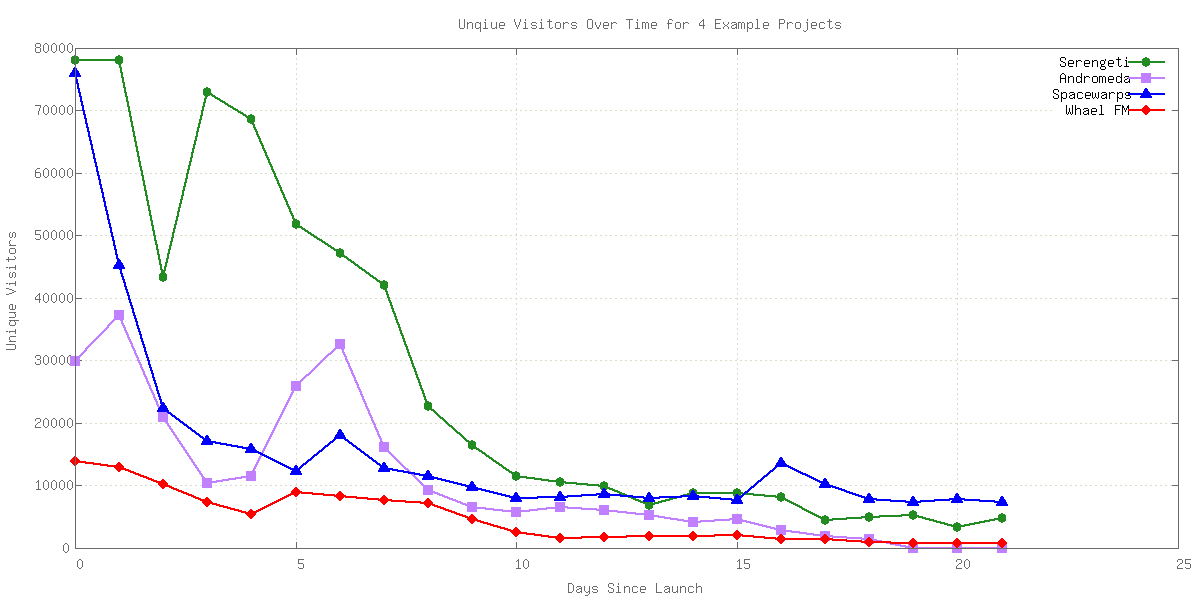
\includegraphics[width=0.48\textwidth]{data/launch-profiles/launch-profiles.png}
\caption{Launch profiles for 4 example Zooniverse projects.}
\label{launchprofiles}
\end{figure}

Shown above in Figure \ref{launchprofiles} are the first three weeks of activity on four Zooniverse projects: Whale FM (Nov 2011), The Andromeda Project (Dec 2012), Snapshot Serengeti (Dec 2012) and Spacewarps (May 2013). Each project displays a subtly different profile of activity in its first days and weeks. % For example ... X and Y .... 

% TODO: Rob - Add annotations to this plot and talk about events that influenced the profiles. Note that the launch iof Serengeti gives Andromed a boost a week in.

%Add annotations to this plot and talk about events that influenced the profiles. Note that the launch iof Serengeti gives Andromed a boost a week in.
\subsubsection{Response from Exisiting Zooniverse Community}

After the launch of every project the whole Zooniverse community is emailed an announcement with an explanation of the project and how to take part. This pre-existing set of users -- who already have a sign-in for any new Zooniverse site -- is often enough to create a sizeable surge in activity in the early days of a project. In cases where no press coverage exists, this initial boost is sometimes crucial in producing useful data. The case of the Andromeda Project is particularly interesting, as this was the Zooniverse's first new space-based project for almost a year and it did not receive significant press coverage. However, the response from the Zooniverse community was so large that it completed its entire requirement of 1.1 million classifications in sixteen days. Similarly, the initial surge in traffic on the Spacewarps project was impressive (10,000 people contributed 500,000 classifications in its first twenty-four hours) and sustained (more than 10,000 people were visiting the site every day even three weeks later), and it took days for blogs and news sites to pick up the project and publish about it more widely.

% http://blog.andromedaproject.org/2013/01/14/first-results-at-aas/ is the source for the change above from "just over two weeks" -> 16 days

\subsection{Sustaining Engagement}

Consistent with visitation patterns to most web sites \cite{TODO}, it was observed that visitors to the Zooniverse apps were increasingly likely to leave the site every passing minute on the site, than to stay.  Moreover, since after a user left, the probability that they would ever return was estimated to be at most an odds ratio of $10-to-1$, maximizing the amount of participation meant engaging users with tasks as soon as they first landed.  This had profound implications on the design of the tutorial, as we describe later, getting users acquainted to the system and their task.  The result of optimising this process, however, did allow a significant amount of contributions to be gathered by short-stayers; ultimately, over half of Zooniverse's classifications were performed by users who only visited the site \emph{once}.

%% immediately was a priority for maximizing the amount of potential participation overall.  Even more the likelihood of a later return to the site was (Over half of the classifications were contributed by users who never returned. This of course, has significant implications 
%% From the very first moment that a user arrives on a website, they are more likely to leave than to stay. The faster they can be engaged with participation in the main (citizen science) task, the more people will have participated over all.
%% % TODO this has a significant implication for the training/tutorial phase for getting new users oriented with their task, as users are likely to leave

A number of factors also seemed to influence the remaining engagement.  First, having a `Call to Action' appears to improve retention; sites with clear, succinct front-page descriptions of a project's intention have lower bounce rates overall (the fraction of people who leave and don't classify). This was first seen clearly with Planet Hunters but also with Galaxy Zoo's fourth incarnation. % TODO: Can we show a visual example of a call to action versus not?

By no surprise, a key factor that sustains participant motivation pertains to interesting-ness of the subjects themselves.  For example, those who witness ``beautiful'' galaxies in Galaxy Zoo, or an image containing interesting animals in Snapshot Serengeti, will stay longer and perform more classifications than those who did not see said images.  To measure this, we identified which subjects were most favourited, and examined whether those users who witnessed these subjects stayed longer, which was significant (Statistical measure). %TODO: Rob please!

% Another key factor seems to be the graspability of the task - (and this can be challenging; for example, Galaxy Zoo is not about discovering galaxies, but documenting galaxy evolution as a function of their geometry) 

A third factor pertains to task difficulty. Projects with innately simple to perform tasks (e.g. Ice Hunters, Spacewarps) show much higher classifications-per-user numbers than projects with more difficult tasks (e.g. Milky Way Project, Cyclone Center). The complexity or difficulty of a task does not appear to be correlated with how long users spend on the site in any session, however; Moon Zoo and the Milky Way Project have similar interfaces but very different dwell times. Conversely, Ice Hunters and Old Weather had similar dwell times for many months, despite one being far more complex than the other.

% Having a clear call-to-action / message
% Feedback: progress TODO: (move up here from down below)

%%   % TODO: can we say anything about the effect of the narrative in Old Weather? 
%%   % evidence in the discussion forums ? 
%%   %   > i wonder why the handwriting has changed?
%%   %   > most keen to help each other out -- 

%% did they create rules - placing limitations to achieving the goal -> make a challenge
%% what feedback system did they use and what was the overall goal
%% icebergs/seal hunting : people really wanted a seal. :( 
%% audio :: 
%% posters vs 
%% adding context: old weather
%% achieving flow state


\subsubsection{Interaction During Classification}
In addition to the above section on tutorials, there are other ways to give users feedback about their efforts in citizen science.

Since Galaxy Zoo 2 there have been occasional project-`ometers' created to show progress of the community toward a common goal or project completion. The Planet Hunters `Planetometer' displays the total number of classifications of the project, as well as the number planet candidates discovered. The `Moonometer' shows the cumulative area of the Moon that Moon Zoo has scoured for craters in various units\footnote{Units include Square Miles, Football Fields, Taj Mahals, Switzerlands, Utahs, Texas, Polands, Wales, Whales and others -- see http://www.moonzoo.org/moonometer}. These counters exist on many projects but not all. When counters were present, participants often noticed when project milestones were being approached, as well as when new subjects were introduced.  In the former, participants sometimes posted messages in the forums pointing out that they were approaching the particular milestone to motivate others to pitch in to help.  In the latter, the addition of new data meant that there was significant new work to be done, and participants occasionally posted messages rallying support for starting on the task.  These ``project-o-meters'' also indirectly seemed to support bringing in  participants by attracting journalists and bloggers who often wrote about projects' progress citing these meters, which, in turn drove further traffic to them. 

% milestone - when they didn't want to finish the logs because they didn't want to finish it off

%% Since Galaxy Zoo 2 there have been occaisional project-`ometers' created to show progress of the community toward a common goal or project completion. The Planet Hunters `Planetometer' displays the total number of classifications of the project, as well as the number planet candidates discovered. The `Moonometer' shows the cumulative area of the Moon that Moon Zoo has scoured for craters in various units\footnote{Units include Square Miles, Football Fields, Taj Mahals, Switzerlands, Utahs, Texas, Polands, Wales, Whales and others -- see http://www.moonzoo.org/moonometer}. These counters exist on many projects but not all.

Where they do exist these counters do not normally appear to drive people to participate, but they do appear to be heavily discussed by people writing about projects and by dedicated users noticing the approach of milestones. In the case of Galaxy Zoo 2 there was a drive toward 60 million classifications in March 2010, to mark the completion of the project; whereas in Old Weather the imminent arrival of `100\% Complete' on the homepage caused users to slowdown and literally ration themselves to abate the project's conclusion.

Individual counters of a single user's classifications have existed for several projects as well as result in people talking about their own classification count. A volunteer's counter for all projects has existed on the the Zooniverse homepage\footnote{http://www.zooniverse.org} for two years but is rarely discussed and in fact many regular users of the site have no idea it is there!

More recent Zooniverse projects have been able to include synthetic or expert data. This has meant that in many cases a user can be given instant feedback on their classification. The reaction to has been almost universally positive, and it appears to give confidence to some users who might otherwise have not continued with the project. The most recent example is Spacewarps, which gives continuous feedback, although at an ever-decreasing rate, throughout a users time on the site.

% In addition to remarks on tutorials, there are other ways to give users feedback about their efforts in citizen science.

%% TODO: Rob: Anything to say about the way we measure engagement? has this changed? 
%% \subsection{Measuring Engagement}

\subsection{Interaction Flow}
% jump straight to action, no introductory video
% start with 1 GS, interleave gold standards w/ real things

\subsubsection{Social Media}
% favouriting, tweeting, blog posts
Often the majority of posts in an online forum are contributed by a minority of active participants, also referred to as the "power law distribution of participation" \cite{lampe2010motivations}. 

% TODO: Move to -------------> out of this section
\subsection{Deployment Constraints on Design}

\subsubsection{Low-Latency Interaction at Scale}
Creating a responsive online environment requires more sophisticated back end technology. Classification subjects must be drawn out of the whole set on a per-user basis (e.g. users should not see the same subject twice). This creates load on the database every time a new user comes to the classification interface. This situation creates a problem with large datasets, where grabbing a random subject could take up to several seconds; a very long time on a website. The need for reduced load times led to the adoption of \emph{Redis} a database/queue system that can deliver random assets quickly. It also prompted a move away from standard \emph{MySQL} databases per-project and toward a unified \emph{MongoDB} datastore.

The combination of \emph{MongoDB} and \emph{Redis} means not-only faster websites, but also allows for more complex subject selection rules. For example, it becomes possible to group-up and prioritise subjects, or vary the number of required classifiers over time. Significantly it has allowed for subjects to be retired from classification if they contain nothing of note. This has hugely improved the issue of projects with intrinsically less-appealing or repetitive datasets.  

% \subsubsection{Other deployment considerations..}

\section{Discussion}

\subsection{Common Myths of Citizen Science}
\subsubsection{Myth $X$: Putting new users through a `tutorial` is a good idea}
\subsubsection{Myth $X$: Experienced / advanced users perform better than new users}
We have seen no support for this hypothesis; in fact an examination of projects ($X$ etc) demonstrated no correlation between duration of use and user performance \cite{simpson2013dynamic}. 

However, there was evidence that the ways that people get better at using the interface, and that they understand what they are doing with the interface better; for example, with Snapshot Serengeti experience users generally migrate from using the more laborious decision tree interface for describing the animal's features to directly identifying the class and species of animal.

\subsubsection{Myth $Y$: Citizen science projects have to be `gameified'}
McGonigal identified four defining elements of a game: a goal, rules, feedback system and voluntary participation. Other features such as leader boards, badges, the `winning' sensation are all used to reinforce these core concepts but do not create a game environment in their own right \cite{mcgonigal2011reality}. To further this gameplay is a state which encourages an optimistic outlook on personal capabilities, partnered with `invigorating rush of activity' \cite{mcgonigal2011reality}. These concepts would support a science citizen, creating a gameplay state to highly motivate and encourage them to undertake difficult challenges. 

%% The team observed that it took a considerable amount of effort to gameify projects and no net gain occurred over simply
%% stating "x is really important/beautiful/whatever and we want to study it/save it, please help." Also, it appears that 
%% for a game to be 'fun' it required an activity which significantly slowed the classification rate, such as in the 'ash game'
%% that Chris and Rob mentioned while in Oxford. Instead, they opted to use Obfuscated Gameification, where aspects of gameification
%% were used, such as leaderboards and badges, to encourage participation, without having overt gameification. In addition, users
%% contribute because of intrinsic motivations such as "I really want to help with science" and their views of what constitutes 
%% science and what satisfies these intrinsic motivations conflict with gameified projects (? - mentioned by people here but not heard from the team)

\subsubsection{Myth $Y$: I should include a 'Don't Know' Button}
% Serengeti blog post - "http://blog.snapshotserengeti.org/2012/12/14/we-need-an-i-dont-know-button/"
% Needs of science/admin team vs desires of users - not having button far more advantageous for science team and can give tag
% subjects even though subject may not be clear - e.g, evidently something small even though not sure what.
% However, talk discussions show that this can lead to misuse of buttons - "nothing here" when there clearly is.
\subsubsection{Myth $Z$: Participants become domain experts}
% Related to a previous myth, in that users don't get more accurate with their classifications, so any expertise gain is just as likely to include 'false' expertise - that is, users might learn something about certain galaxies, while simultaneously learning fallacies about other galaxies, in which case they can hardly be said to be experts.
\subsubsection{Myth $Z$: Beautiful pictures are necessary}
% Planet Hunters popular, but lacks pictures - In fact uses graphs, which could hardly be called beautiful
\subsubsection{Myth $Z$: Non-pictorial data are harder to understand}
% Planet Hunters uses graphs but users do not need to understand the whole graph to classify - Only to identify transit features
\subsubsection{Myth $Z$: Images don't have to be beautiful and graphs don't have to be scary)}
There was an initial fear during the development of Planet Hunters that showing participants the light curves as infographics would result in less participation (either by turning participants away from the task) or would simply be unable to perform the task because of being unable to understand what the data represented.  Planet Hunters has been shown, however, just the opposite, and is one of the most successful apps overall.  
\subsubsection{Myth $Z$: The Data Aren't 'Good Enough'}
\subsubsection{Myth $Z$: If You Build It, They Will Come}

It is a common misconception that websites are busy by default. It should go without saying that publicity and attention are required for people to find an online citizen science project. Networks and communities exist online to allow people to discover and share online projects. The Zooniverse was one of the first organisations in this field and has grown a substantial network of people around it (\~860,000 at time of writing).

However above simple awareness, any creator of a citizen science project should be aware of the approximate effort required. Most Zooniverse sites enlist the help of tens of thousands of online volunteers. Thus when projects are designed, consideration should be given to the scale of the endeavour being attempted. Taking into account a reasonable expectation of web traffic and the effort any person may put in is difficult (how long is a piece of string?) but important for establishing a project with a realistic end goal within the required time. Simply producing a citizen science website does not guarantee popularity -- or more importantly scientific completion of the intended task.

% Zooniverse projects draw a substantial number of contributors from the pre-existing community - See Andromeda Project mentioned above, completed in sixteen days due to pre-existing community being informed by newsletter. 
% Without this community, would have taken much longer. Difficult to form community without 'luck' - Sky at Night and media plugs for various projects, for example, more down to who is on the team. Certainly not users flocking to Zooniverse just because it exists.

\subsubsection{Myth $Z$: Moderator involvement encourages discussion}
% comments from Rob and Chris?

Studies conducted in the educational sector have discovered that contrary to popular belief, instructors (i.e. experts) who contribute often to discussions actually decreased student posts \cite{zydney2012creating}. However, Mazzolini and Maddison propose that this reduction could be a result of more efficient discussion and understanding \cite{mazzolini2007jump}. 

In a forum context, an interactive post is one which responds or replies to another's message, whereas a participation is the number or length of a post \cite{schrire2006knowledge}. 
Schrire discovered two distinctive interaction patterns: instructor-centered, messages predominantly responded to the post by the instructor and synergistic, student-student collaboration \cite{schrire2006knowledge}. 

\subsection{What makes a good citizen science project?}
\subsubsection{Design Builds Trust}
% \subsection{Scaling/latency and practical deployment constraints during design}

\subsection{Comparison to Other Systems}
% Comparison with Jeremy Bentham project - failed in the sense that required more energy than was gained out of it, 20 people at the end
% YourPaintings
% Be A Martian
% FoldIt

% \subsection{A Heuristic Framework for Citizen Science App Designers}

%% In order to put the observations described above into a more concise, easily communicated and form, we assembled common themes into a multidimensional framework of design heuristics for citizen science system designers, comprising 6 constructs, described below.  Each construct is meant to address a key dimension of the necessary components described earlier, using the observations discussed in findings. The purpose of such a framework is intended both as an artefact for discussion and refinement, and potential practical use by designers seeking to apply insights from the Zooniverse team  currently made by the Zooniverse team.

% attracting new users' attention / expanding the user base
% identifying 'good' projects - understanding what can be turned into a good Citizen Science project
% contextualising the project
%   interestingness/difficulty/conceptual+contextual+narrative threads that tie the tasks together/understand the point of it
%
% performing the task - 
%   - tutorials
%   - elicitation/task vtrtvgtvvt4interface considerations // wide open, specific labeling, decision trees
%   - levels of design and their considerations (aesthetics, challenge, interestingness)
% discussion and collaboration - 
% retaining experienced + most valuable participants
% dealing with new data ~
% distilling knowledge from contributions : (amalgamating responses into thing)

% other/misc
%   transferring interest to other projects
% almost always needs a discussion space
\subsection{Engagement: Interestingness x Difficulty x Context}

\section{Future Work: Zooniverse and Citizen Science}

\subsection{Involving citizens in article authoring}

Given the \emph{Voorwerp}, \emph{Green Peas}, \emph{Convict Worm} and other examples of citizen engagement beyond classification, one of the key areas is expanding the role of citizens beyond classification, to that of partners in a scientific collaboration.  To do this, the Zooniverse team has launched a new project and associated tools called \emph{Zooniverse Quench}\footnote{Zooniverse Quench \url{http://quench.zooniverse.org}} which 
%% Quench early observations

%% FUTURE WORK
%% AUTOMATIC ONSET DETECTION FOR scientists
%% REPUTATION system - where there was someone who was very well spoken and loud, and writing technically
%% people have their own categorisation
%    if you email them they will be overload
%    SO, catch scientists them when they go to the site> CHECK OUT THIS DISCUSSION THREAD

% A-B testing alternatives - the cost of deriving two designs and 
% formally A-B testing them can be prohibitively expensive

\section{Related work}

\section{Conclusion}

\section{Acknowledgments}
Acknowledgments omitted for blind review.

\balance

%% elena notes
%%   actual task - functionality - the button was missing/feature was missing
%%   tutorial how do we teach them
%%   discussions
%%   launching projects
%%   sustaining engagements
%%     direct feedback
%%     effect of latency change on engagement?

%%   -----------
%%   punt :: deployment constriants on design  -- this is a real time systems
%%     and there are some specific feature sthat really need to go quickly
%%     it turned out that this combination worked well....
%%     any deployment engineer would have been able to figure out 

%% The Zooniverse framework team has derived significant has
%% been successively refined and scaled as the variety of tasks and
%% number of participants have increased.  At its current state,
%% currently having launched $X$ distinct applications for $Y$ scientific
%% domains, including astronomy, zoology, cell and marine biology,
%% archaeology and paleontology.  This platform represents a unique\cite{moore2011facebooking}


%%  These
%% applications, though separate, have been built on top 

%% The experiences from the first were used to derive design goals for
%% the next,

%% The contributions of the 
%% We identify key design challenges

%% especially as the best practices for designing citizen science systems
%% has not yet emerged.  Among the many design challenges include, being
%% able to appeal to participants with an extremely wide range of
%% expertise, ranging from no knowledge of the field to significant
%% background and interest.  Participants naturally feature a diversity
%% of natural competencies, which is manifested in some people being
%% simply much more adept at some tasks than others. Second, people have
%% many different reasons for engaging with citizen science projects, and
%% to sustain engagement, these platforms must appeal to, and engage
%% these different motivating reasons. Finally, there are a large variety
%% of issues pertaining to individual retention, well as supporting
%% various degrees of engagement -- from the ``sunday scientist'' to the
%% ``scienceoholic''.


%% The purpose of this examination of Zooniverse is to both to document
%% the experience gained from launches and iterations of the various
%% applications, comparing these experiences against previously
%% documented in other citizen-science projects.  The observations derive
%% from a lateral examination of the

%% The path from its first experimental app, Galaxy Zoo, to the 
%% twenty seven different projects that have launched on the Zooniverse project
%% required generalising the findings from the first project to different
%% kinds of tasks in other scientific domains.

%%  naturally Participants come from a wide
%% audience % with a massive variety of backgrounds and competencies,
%% such systems interface down to the workflow of how participants' input
%% is collated, verified, and provided as feedback to the participants,
%% along with the nature and kind(s) of affordances provided for
%% communicating and discussing remains challenigng

%% interfaces that have
%% appropriate affordances, the and features remains challenging, due
%% to the wide number of design considerations that mustbe taken
%% jointly into account.

%% Wide variety of expertise

% \section{Background: Brief History of Zooniverse}

% \emph{For the CSCW readers, outline the history of the development of the system
% including a detailed description}

% \section{Observations through iterations}

% \emph{I was thinking put key design observations here relating to how to cross-domain
% citizen science}

% If you want to use smaller typesetting for the reference list,
% uncomment the following line:
% \small


\bibliographystyle{acm-sigchi}
\bibliography{zooniverse-history}
\end{document}

%% from crw04
%% \begin{algorithm}[tb]
%%   \caption{Overview of our general negotiation process, which is common to all of our strategies.  Let $o_\text{own}$ and $o_\text{opp}$ represent our own and the opponent's latest offers, respectively. $t_c$ is the current time and $u_\tau$ is the aspiration level at time $t_c$.}\label{alg:generic-overview}
%%   \begin{algorithmic}
%%     \FOR{$t_c \in [0,1]$}
%%     \STATE $o_\text{opp} \Leftarrow $ {\sc ReceiveOffer}()
%%     \STATE $u_\tau \Leftarrow $ {\sc SetAspirationLevel}($o_\text{opp}, t_c$)
%%     \IF{{\sc GetUtility}($o_\text{opp}, t_c$) $\geq u_\tau$}
%%     \STATE {\sc AcceptOffer}($o_\text{opp}$)
%%     \RETURN
%%     \ENDIF
%%     \STATE $o_\text{own} \Leftarrow $ {\sc GenerateOffer}($u_\tau$)
%%     \STATE {\sc ProposeOffer}($o_\text{own}$)
%%     \ENDFOR
%%     \end{algorithmic}
%% \end{algorithm}

%%  LocalWords:  artefacts HCI artefact Dropbox Skydrive Google PDF
%%  LocalWords:  LaTeX versioning throughs interactional CDSSes UI LD
%%  LocalWords:  bioinformaticians iPad iCloud iCal favour favourite
%%  LocalWords:  microformats picoformats WebDAV situ VCS scm priori
%%  LocalWords:  Powerpoint CB's CBs each's bulleted parseable OTs
%%  LocalWords:  sub-schemas pre Dourish XLSX csv PPTX PPT ICS CalDAV
%%  LocalWords:  RSS VCF XSLT XLST CSS Dojo PNG


%% notes from Oxford, 22 August
%% SOCIAL MEDIA  > 
%% troubleshooting >> social media is used for troubleshooting
%% source of traffic >> we get a significant amount of traffic from social media
%%  whale.fm gets a lot of traffic from social media

%% INTERFACE >
%% Rising percent of tablet users > it needs to work on an ipad
%%  - ones that promote on the telly

%% Discussion forums >
%%    Why they were introduced
%%    How it evolved and emerged
%%       From "What's this?" to so much more!
%%       Increase engagement by letting people share pretty galaxies and discuss
%%        (basic statistics of how many people have done this)
   Key players / decisions - Moderators
%%       Independently tested hypothesis and moderators emerged as key mediators between participants and scientists
%%     Peas and verpwork 
%% Questions for Chris::
%%    _Key affordances of the forums w.r.t. how they facilitated these discussions_
%%    _Missing affordances - things that would have helped_
   _Role of project managers and scientists_
%%     What did they do to make things happen
%% Two path to science
%%   -> show -> classifications
%%           -> interesting things to talk about


  
